\documentclass{ximera}
\graphicspath{{./content/hw_01_coordinates/graphics/}{./graphics/}}
\title{Homework 1: Coordinates}
\begin{document}
\begin{abstract}
\end{abstract}
\maketitle

\section*{Graded Problems}

\begin{problem}
Consider the surface in $\mathbb{R}^3$ described by the equation $(r-2)^2+z^2=1$ in cylindrical coordinates.
\begin{enumerate}
\item Sketch the intersection of this surface with the $xy$-plane.
\item Given that $\theta$ does not appear in the equation, what can you say about the surface?
\item Sketch the surface.
\end{enumerate}
\end{problem}

\begin{problem}
\begin{enumerate}
\item Suppose we have a curve in $\mathbb{R}^2$ defined by the polar equation $r=f(\theta)$, for some function $f$. What is the relationship between this curve and the curve defined by $r=f(\theta+\pi/4)$ in polar coordinates?
\item Suppose we have a surface in $\mathbb{R}^3$ defined by the cylindrical equation $r=g(\theta, z)$, for some function $g$. What is the relationship between this surface and the surface defined by $r=g(\theta + \pi/4, z)$ in cylindrical coordinates?
\item Suppose we have a surface in $\mathbb{R}^3$ defined by the spherical equation $r=h(\theta, \phi)$, for some function $h$. What is the relationship between this surface and the surface defined by $r=h(\theta + \pi/4, \phi)$ in spherical coordinates?
\item Again, suppose we have a surface in $\mathbb{R}^3$ defined by the spherical equation $r=h(\theta, \phi)$, for some function $h$. What is the relationship between this surface and the surface defined by $r=h(\theta,\phi+\pi)$ in spherical coordinates? \emph{Hint: it's not a rotation.}
\end{enumerate}
\end{problem}

\section*{Professional Problem}

\begin{problem}
Consider the solid below, which is obtained by taking the portion of a solid sphere of radius $2$ which is outside of the (double) cone $z^2 = x^2+y^2$.

\begin{image}
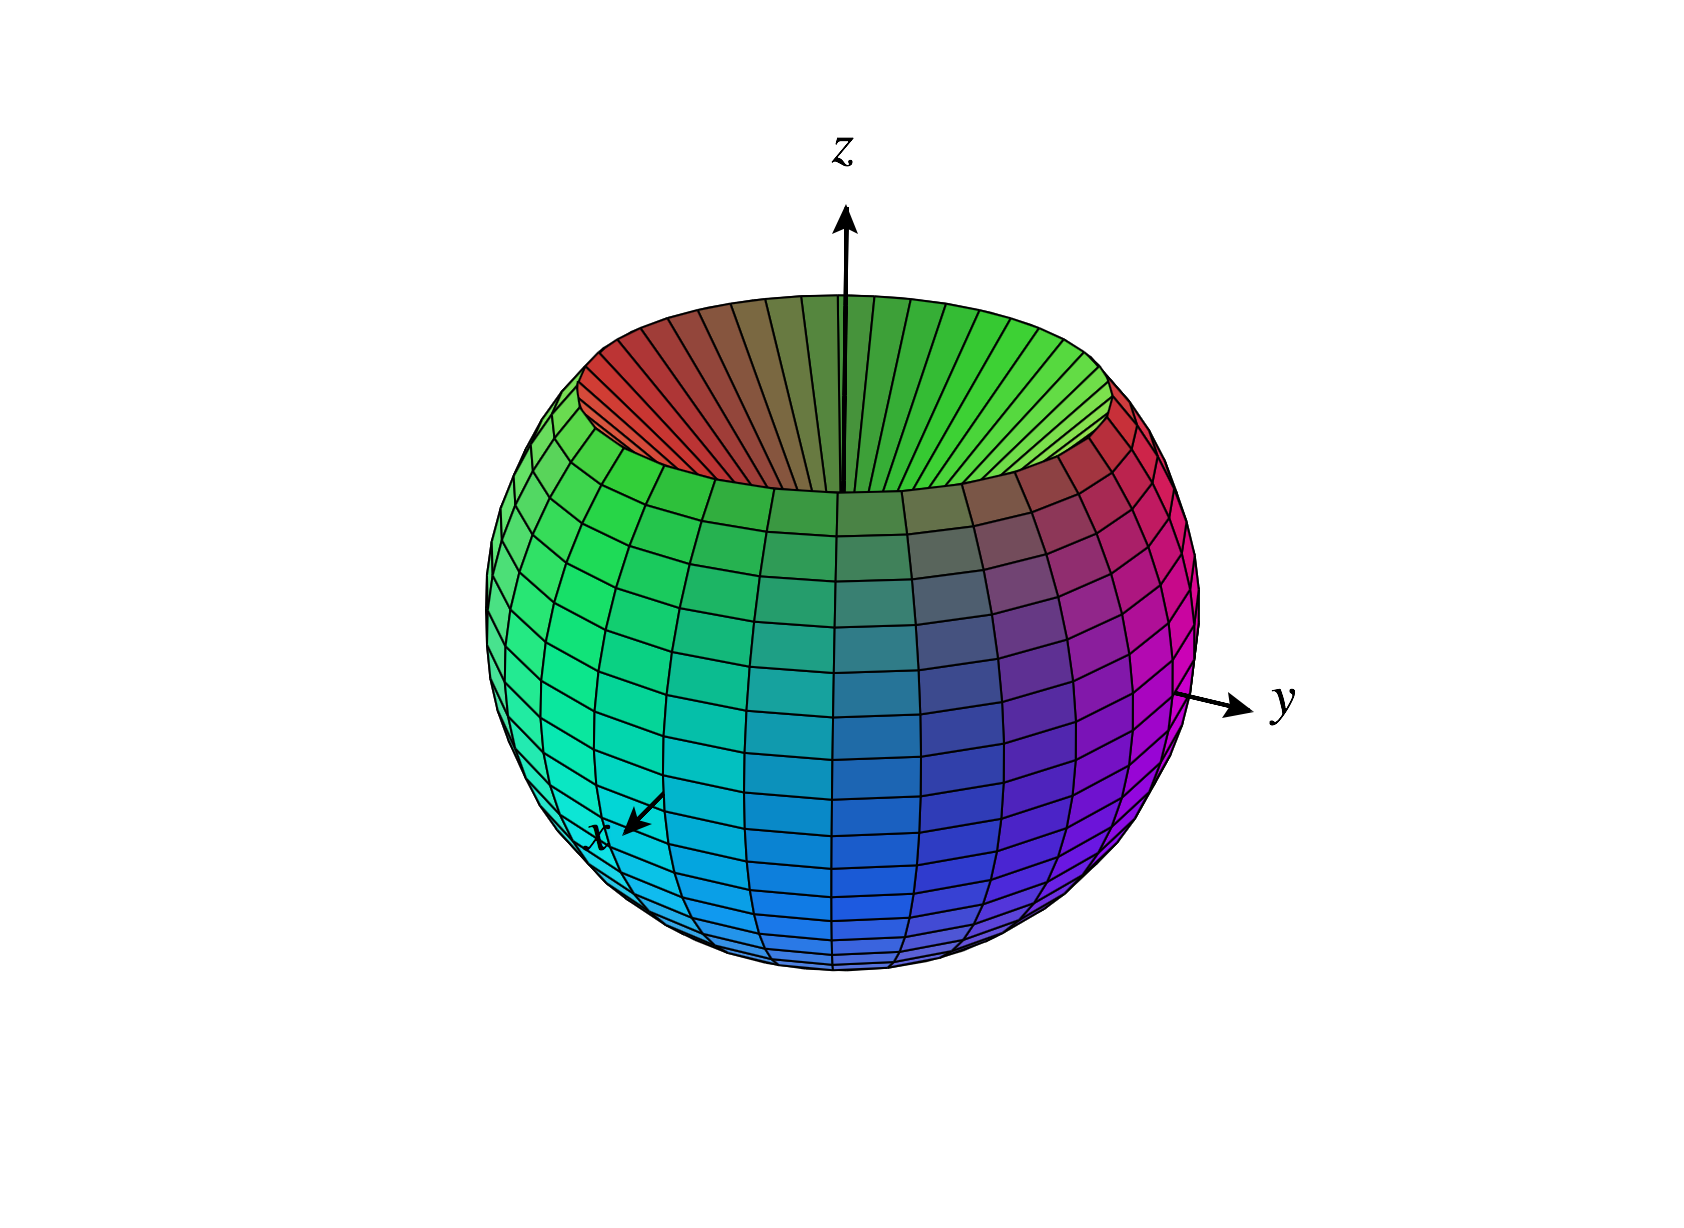
\includegraphics[width=\textwidth]{CalcPlot3D-pp_1}
\end{image}
\begin{image}
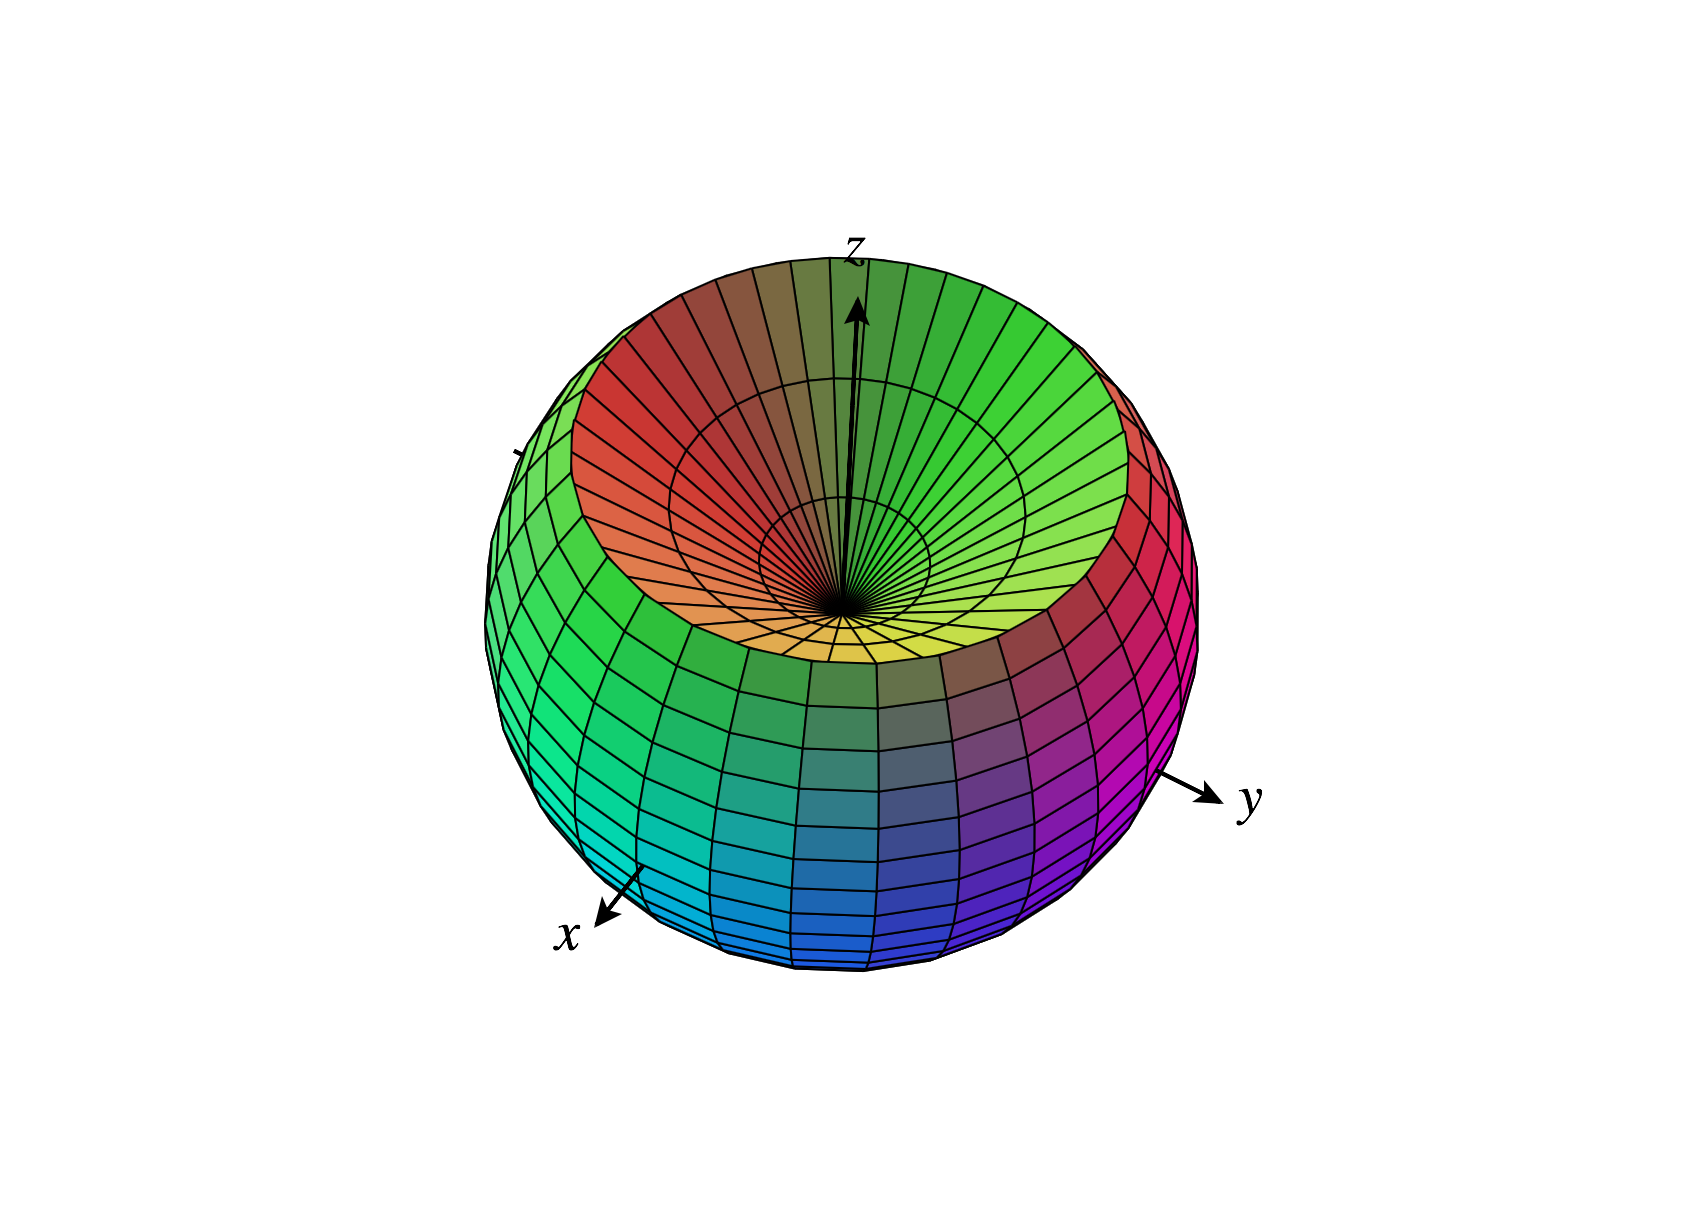
\includegraphics[width=\textwidth]{CalcPlot3D-pp_3}
\end{image}
\begin{image}
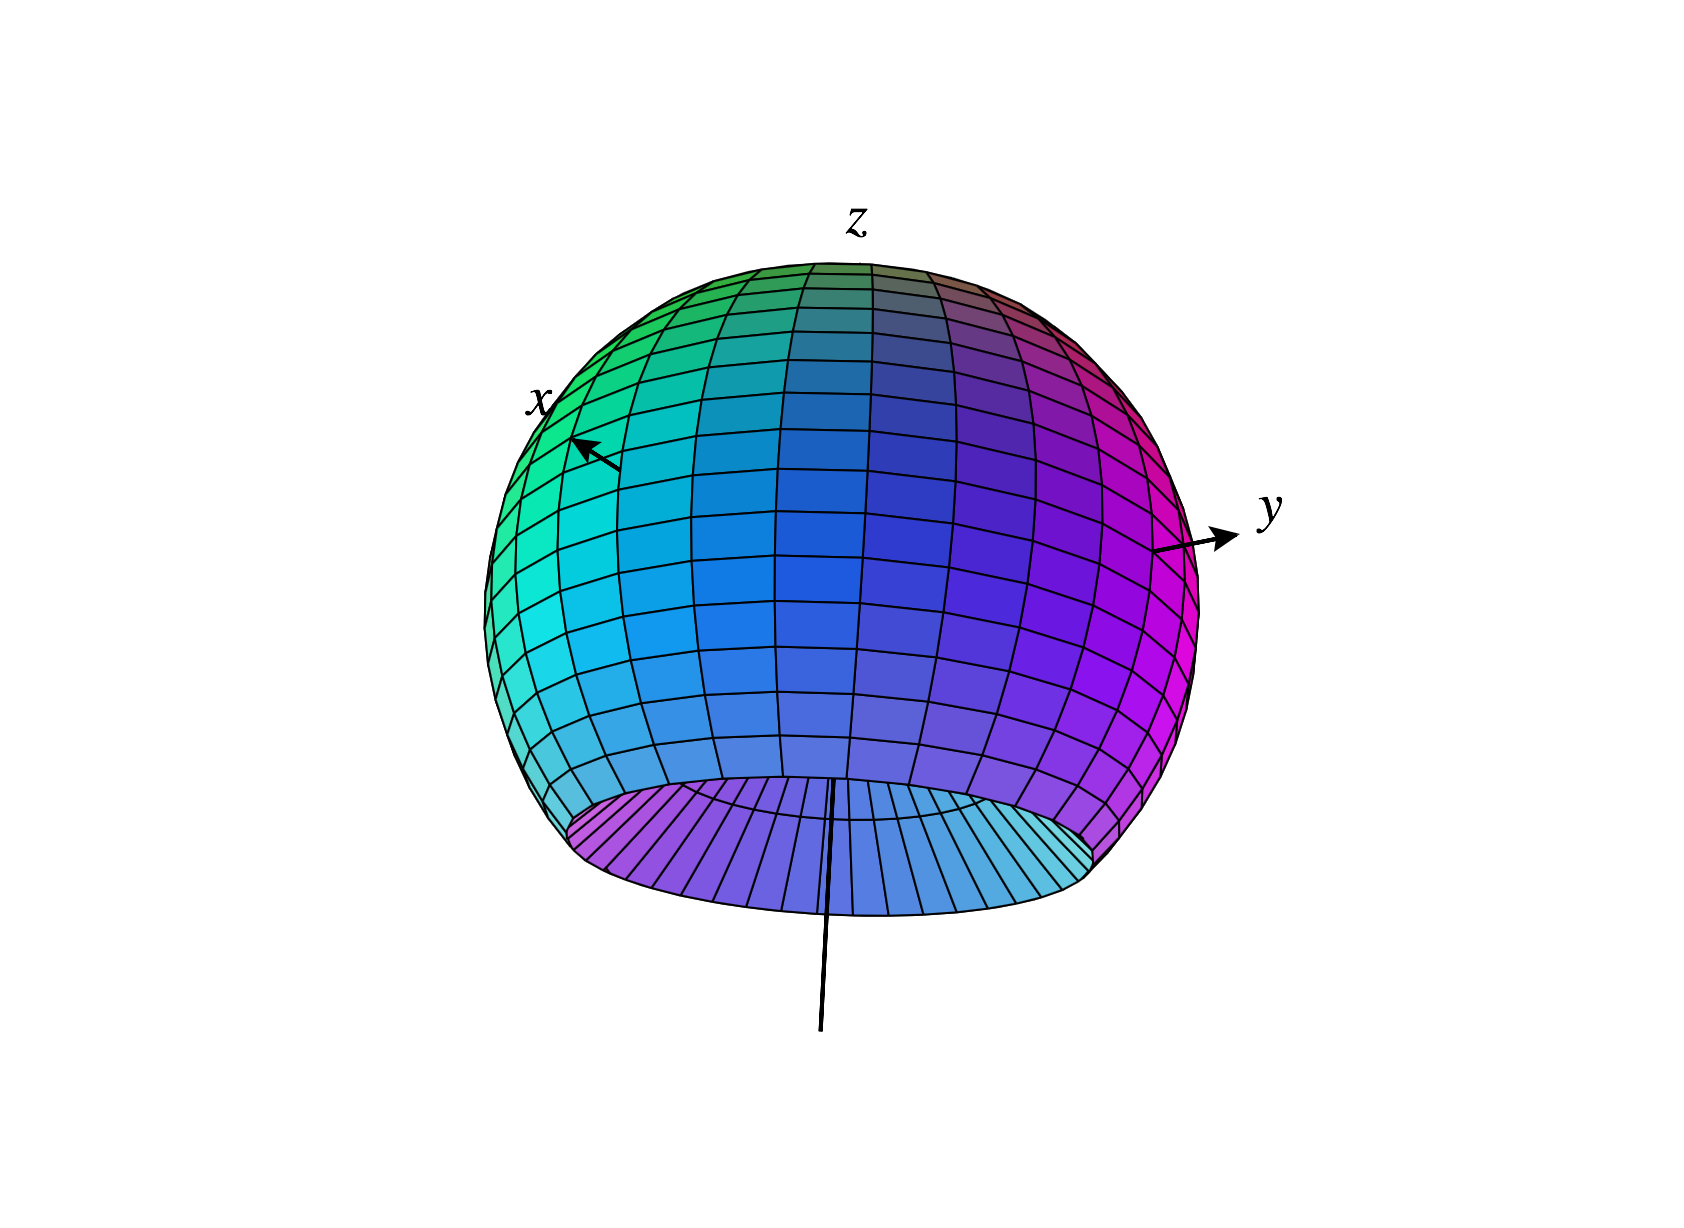
\includegraphics[width=\textwidth]{CalcPlot3D-pp_2}
\end{image}

\begin{enumerate}
\item Is this region easier to describe in spherical coordinates or in cylindrical coordinates? Justify your answer.
\item Describe this region in either spherical coordinates or cylindrical coordinates (based on your answer to (a)).
\end{enumerate}

\end{problem}

\section*{Completion Packet}

\begin{problem}
Consider the point $P=\left(\frac{\pi}{4}, \frac{\pi}{4}, \frac{\pi}{4}\right)$, given in crylindrical coordinates. What are the Cartesian coordinates of $P$?
\end{problem}

\begin{problem}
Consider the point $P=\left(\frac{\pi}{2}, \frac{\pi}{2}, \frac{\pi}{2}\right)$, given in spherical coordinates. What are the spherical coordinates of $P$?
\end{problem}

\begin{problem}
Consider the point $P = (2,1,3)$, given in Cartesian coordinates. Find all possible ways to write $P$ in cylindrical coordinates.
\end{problem}

\begin{problem}
Consider the point $P = (2, 1, 2)$, given in Cartesian coordinates. Find all possible ways to write $P$ in spherical coordinates.
\end{problem}

\begin{problem}
Sketch the graph of the surface in $\mathbb{R}^3$ defined by the equation $\rho = \cos(\phi)$ in spherical coordinates, for $0\leq \phi\leq \pi$.
\end{problem}

\begin{problem}
Consider the surface in $\mathbb{R}^3$ defined by the equation $2x^2+2y^2+z^2=1$ in Cartesian coordinates.
\item Convert the equation to cylindrical coordinates.
\item Convert the equation to spherical coordinates.
\item Sketch the surface.
\end{problem}

\begin{problem}
Sketch the region defined by the inequalities $\pi/4\leq \theta\leq \pi$, $0\leq r\leq 2$, and $0\leq z\leq r$ in cylindrical coordinates.
\end{problem}

\begin{problem}
Sketch the region defined by the inequalities $0\leq \phi\leq \pi$, $0\leq \theta\leq \pi$, and $0\leq \rho\leq \theta$.
\end{problem}

\begin{problem}
Consider the region defined by the inequalities $0\leq r\leq 1$, $0\leq \theta \leq 2\pi$, and $0\leq z\leq 2$ in cylindrical coordinates.
\begin{enumerate}
\item Sketch this region.
\item Describe this region in spherical coordinates.
\end{enumerate} 
\end{problem}


\end{document}